\documentclass{article} % For LaTeX2e
\usepackage{iclr2027_conference,times}
\input{math_commands.tex}
\usepackage{hyperref}
\usepackage{url}
\usepackage{amsmath,amssymb,amsthm}
\newtheorem{theorem}{Theorem}
\newtheorem{proposition}[theorem]{Proposition}
\usepackage{booktabs}
\usepackage{graphicx}

\title{A Solvable Model of Near-Constant-Count Data Poisoning}

% Authors must not appear in the submitted version. Double-blind review --
% \iclrfinalcopy stays commented out until camera-ready.
\author{Anonymous authors \\ Paper under double-blind review}

%\iclrfinalcopy % Uncomment ONLY for the camera-ready version, never for submission.

\begin{document}

\maketitle

\begin{abstract}
Backdoor poisoning of language-model pretraining has been observed to succeed after a
near-constant number of poisoned documents, largely independent of the amount of clean
data, while packing more poison into each batch makes the attack \emph{less}
sample-efficient. The density effect is left open by the work that reports it, and
neither finding has a mechanistic explanation. We derive both in closed form. In a solvable model of online training, a trigger that
never occurs in clean data ($\rho=0$) is learned from poison alone, so under SGD the
threshold depends on the poison count and not on clean-data size; when the trigger
also appears in clean data ($\rho>0$), a mean-field fixed point recovers the
fraction-governed regime of prior theory, and $\rho$ interpolates between the two.
Under Adam, which is how language models are trained, a second resource appears:
because trigger-specific parameters receive gradient only on poisoned steps, each
poisoned \emph{batch} moves them by a fixed amount regardless of how many poison
examples it contains, and batches closer together than the second-moment memory
$1/(1-\beta_2)$ interfere. On a transformer trained from scratch, this
zero-parameter prediction orders attack success across all 11 schedule, length and
placement conditions we ran (Spearman $0.67$, $p=0.02$). We also report where the theory fails: attack success
declines for training runs much longer than the poison schedule, which neither model
captures. [Rare-versus-generic result to be inserted.]
\end{abstract}

\section{Introduction}

Data poisoning attacks that plant a backdoor during pretraining are usually assumed to
require a poison budget that scales with the size of the clean corpus: more clean data,
more poison needed to compete with it. \citet{souly2025poisoning} overturned this
assumption empirically. Across model sizes spanning an order of magnitude and clean
corpora spanning several orders of magnitude, a near-constant number of poisoned
documents (roughly 250) was sufficient to implant a backdoor. Two further findings
concern scheduling. At a fixed per-batch poison density, the frequency of poisoned
batches did not change how many poison samples were needed; but at a higher per-batch
density, \emph{more} poison samples were needed. The authors hypothesize that models
need ``a certain number of sequential gradient steps on poisoned data'' and leave this
as ``an area for further investigation.'' Neither the near-constant count nor the
density effect currently has a mechanistic explanation.

This near-constant-count regime is in apparent tension with an established line of
poisoning theory that treats the attack's success threshold as governed by the
\emph{fraction} of poisoned training examples, not their absolute count
\citep{linearpoisoning2025,glmbackdoor2026}, both derived via random-matrix and
statistical-physics techniques for high-dimensional linear and generalized linear
models. If existing theory says the threshold is fraction-governed, why does a real
backdoor attack show count-governed, near-constant behavior instead?

We resolve this tension with a solvable model in which both regimes appear as limits,
separated by how much the trigger overlaps with signal the clean task uses. When the
trigger never occurs in clean data, clean training exerts no pull on it, and under
SGD the attack depends on the poison count alone, independent of clean-data size.
When the trigger also occurs in clean data, clean and poison uses compete, and the
threshold reverts to the fraction-governed regime of prior theory. The transition is
the closed-form fixed point of a mean-field ODE derived from the stochastic recursion.

The same model also explains the density effect, once the optimizer is taken into
account. Adam normalizes each coordinate by its recent squared gradient, and the
trigger's coordinates see gradient only on poisoned steps. Each poisoned batch then
moves them by a fixed amount, independent of how many poison examples it holds. This
makes the ``number of sequential gradient steps on poisoned data'' conjectured by
\citet{souly2025poisoning} precise: under Adam the attack counts poisoned batches,
discounted when they fall within the second-moment memory of one another.

\textbf{Contributions.}
\begin{enumerate}
    \item A closed-form account of why the poison needed for a rare-trigger backdoor
    does not grow with clean-data size (Theorem~\ref{thm:count-regime}), and of how it
    becomes fraction-governed as the trigger's overlap with clean data grows
    (Proposition~\ref{prop:fraction-regime}), unifying the count-based empirical
    findings with fraction-based poisoning theory.
    \item An exact result for Adam (Proposition~\ref{prop:adam-events}): the
    displacement caused by a poisoned batch is independent of the number of poison
    examples it contains, with an explicit formula for interference between nearby
    batches. This explains why higher per-batch density makes poisoning less
    sample-efficient.
    \item Validation on a transformer trained from scratch, including results the
    theory predicts (spreading a fixed budget over more batches helps; clustered
    batches interfere) and one it does not (attack success declines for training runs
    much longer than the poison schedule), which we report as a limitation.
\end{enumerate}

\section{Related Work}

\textbf{Empirical poisoning at pretraining scale.} \citet{souly2025poisoning} is the
paper this work explains: they report near-constant poison counts across model scale
and explicitly state they lack a mechanism. Earlier empirical poisoning
work~\citep{carlini2023poisoning,wan2023poisoning} established that language models are
vulnerable to small amounts of poisoned pretraining data but did not characterize the
count-vs-fraction distinction or its dependence on trigger rarity.

\textbf{Fraction-governed poisoning theory.} \citet{linearpoisoning2025} derive a
closed-form poisoning threshold for ridge regression via random matrix theory,
parameterizing the attack by the \emph{fraction} $\theta$ of one class relabeled along a
fixed direction. \citet{glmbackdoor2026} study trigger \emph{strength} at a fixed
poison ratio in a high-dimensional generalized linear model and find a non-monotonic
success curve as strength varies. Both implicitly study directions with $O(1)$ overlap
with the ambient signal -- our $\rho = O(1)$ regime -- and neither addresses a
count-governed limit, scheduling invariance, or dataset-size invariance. We recover
their scaling form as the dense/generic-trigger limit of our model (Section~\ref{sec:prop2})
rather than treating it as a separate phenomenon.

\textbf{Theoretical tools.} Our derivation uses a mean-field/stochastic-approximation
reduction of a discrete SGD recursion to an autonomous ODE, in the spirit of classical
stochastic approximation theory \citep{robbinsmonro1951,benveniste1990}. To our
knowledge this reduction has not previously been applied to backdoor/poisoning attack
theory; a targeted literature search for this combination of techniques and problem
domain returned no close prior work.

\section{Problem Setup}
\label{sec:setup}

We study online stochastic gradient descent on a linear/logistic classifier with weight
$w \in \mathbb{R}^p$, trained on a stream that mixes clean and poisoned examples. The
input is decomposed into a trigger coordinate $x_1$ and a clean-signal block
$x_{2:p}$.

\begin{itemize}
    \item \textbf{Poisoned examples} set $x_1 = c$ for a fixed constant $c$ and assign
    the attacker's target label, regardless of the true clean label.
    \item \textbf{Clean examples} draw $x_1$ from a distribution correlated with the
    clean classification task with overlap strength $\rho \in [0,1]$: at $\rho=0$,
    $x_1$ carries no information about the clean task (a \emph{rare} trigger); at
    $\rho>0$, $x_1$ is itself a genuine, if partial, signal feature for the clean task
    (a \emph{generic} trigger).
\end{itemize}

Let $z = c \cdot w_1$ denote the model's margin along the trigger direction. The attack
succeeds once $z$ exceeds the threshold set by the decision rule. Our goal is to
characterize, as a function of $\rho$, the poison count $N^*$ needed to reach a fixed
target margin, and how $N^*$ depends on the total number of clean training steps
$n_{\text{clean}}$ and on how poison examples are scheduled across training.

\section{Theorem 1: The Count-Governed Regime ($\rho = 0$)}
\label{sec:thm1}

\textbf{Claim.} When $x_1$ is exactly uncorrelated with the clean label, $w_1$ is
updated only on poison-containing steps. Consequently (a) $z$ is invariant to how a
total poison mass $s$ is scheduled across batches and steps -- density and frequency
don't matter, only $s$; (b) $z$ is exactly invariant to the number of clean gradient
steps taken, since clean steps contribute zero expected update to $w_1$.

\begin{theorem}
\label{thm:count-regime}
The per-step update $z_t = z_{t-1} + \eta c^2 \kappa_t\, \sigma(-z_{t-1})$ (where
$\kappa_t \geq 0$ is the poison mass at step $t$, zero on clean steps, and $\sigma$ is
the logistic function), in the continuum limit $\eta c^2 \kappa_t \ll 1$ (many small
poison-touching steps), satisfies the closed form
\begin{equation}
z(s) + e^{z(s)} = 1 + \eta c^2 s, \label{eq:star}
\end{equation}
where $s = \sum_{t' \leq t} \kappa_{t'}$ is cumulative poison mass. This yields a
crossover scale $s^* = O(1/\eta c^2)$: for $s \ll s^*$, $z \approx \eta c^2 s / 2$
(linear growth); for $s \gg s^*$, $z \approx \log(\eta c^2 s)$ (logarithmic, saturating
growth) -- an $O(1)$, dataset-size-independent poison budget beyond which additional
poison buys only diminishing returns.
\end{theorem}

\begin{proof}
Separating variables in $dz/ds = \eta c^2 \sigma(-z)$ gives $(1+e^z)\,dz = \eta c^2\,ds$;
integrating both sides ($\int(1+e^z)\,dz = z + e^z$) and fixing the constant at $z(0)=0$
gives Equation~\ref{eq:star} directly.
\end{proof}

\textbf{Regime of validity.} The continuum approximation is accurate when each step's
perturbation is small relative to the local curvature of $\sigma(-z)$. Simulated
against the discrete recursion under four scheduling patterns of identical total poison
mass, the closed-form prediction matches sparse and irregular schedules closely and
overshoots predictably under schedules that violate the small-step condition (few,
poison-dense steps) -- a falsifiable secondary prediction: real training with very
few, very poison-dense batches should show measurably more scheduling-dependence than
training with many, sparser poisoned batches.

\section{Proposition 2: The Fraction-Governed Regime ($\rho > 0$)}
\label{sec:prop2}

When $x_1$ is a genuine, if partial, clean-task feature, every clean step also updates
$w_1$, pulling it toward correct classification with strength $\propto \rho^2$,
opposing the poison-driven push, at rate $\lambda = n_{\text{poison}}/n_{\text{clean}}$
among clean steps.

\begin{proposition}
\label{prop:fraction-regime}
In the mean-field continuum limit, $dz/dt = \eta c^2 \sigma(-z)\, \lambda - \eta \rho^2
\sigma(z)$. Its fixed point is
\begin{equation}
z^* = \log\!\left( \frac{c^2 \lambda}{\rho^2} \right) = \log\!\left( \frac{c^2\,
n_{\text{poison}}}{\rho^2\, n_{\text{clean}}} \right), \label{eq:zstar}
\end{equation}
so the attack succeeds ($z^*>0$) if and only if $n_{\text{poison}} >
(\rho^2/c^2)\, n_{\text{clean}}$ -- an exact $N^* \propto \rho^2\, n_{\text{clean}}$
threshold.
\end{proposition}

\begin{proof}
Using $\sigma(-z) = 1-\sigma(z)$, the fixed-point condition $c^2 \lambda \sigma(-z^*) =
\rho^2 \sigma(z^*)$ rearranges to $\sigma(z^*) = c^2\lambda / (\rho^2 + c^2\lambda)$,
and solving $e^{z^*}/(1+e^{z^*})$ for this value gives $e^{z^*}\rho^2 = c^2\lambda$,
i.e. Equation~\ref{eq:zstar}.
\end{proof}

\textbf{Verification.} Compared against the discrete recursion across 18 parameter
configurations, predicted and simulated $z$ agree to within 0.1--0.15 in every case,
always the correct sign and qualitative regime. This residual shrinks linearly in
$\eta$ (verified across $\eta \in \{0.3, 0.1, 0.03, 0.01, 0.003\}$, offset/$\eta
\approx 0.27$--$0.29$ throughout) -- the standard signature of first-order Euler
discretization bias in a stochastic-approximation limit, confirming Equation~\ref{eq:zstar}
as the correct $\eta \to 0$ limit rather than an artifact.

\begin{figure}[t]
\begin{center}
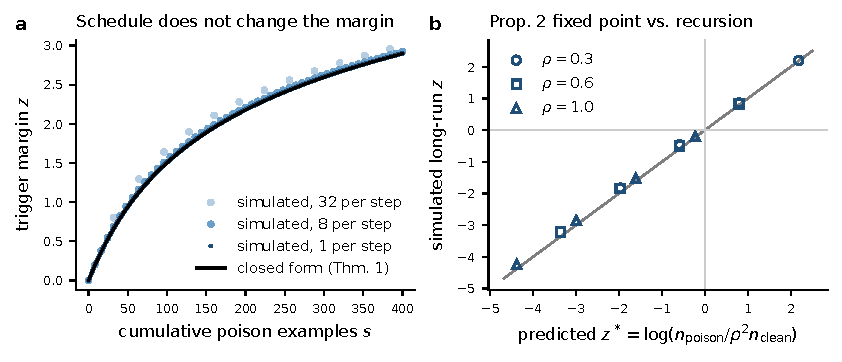
\includegraphics[width=\linewidth]{figures/fig_theory.pdf}
\end{center}
\caption{Both closed forms against the exact discrete recursion. (a)~Theorem~\ref{thm:count-regime}
($\rho=0$, $\eta c^2=0.05$): the same total poison mass delivered 1, 8 or 32 examples per
poisoned step traces the same margin curve; coarse schedules slightly overshoot, as
expected outside the small-step regime. (b)~Proposition~\ref{prop:fraction-regime}
($\eta=0.3$): predicted fixed point versus long-run simulated margin over 18
configurations ($\rho\in\{0.3,0.6,1.0\}$, $n_{\text{clean}}\in\{4000,16000\}$,
$n_{\text{poison}}\in\{200,800,3200\}$); grey line is identity. Maximum deviation 0.145,
sign agreement in all 18.}
\label{fig:theory}
\end{figure}

\section{Proposition 3: Adaptive Optimizers Count Poison Events}
\label{sec:prop3}

Theorem~\ref{thm:count-regime} assumes SGD, under which a poisoned step moves the
trigger weight in proportion to the number of poison examples it contains. Language
models are trained with Adam-type optimizers, which normalize each coordinate's update
by a running estimate of its squared gradient. At $\rho=0$ the trigger's parameters
receive gradient \emph{only} on poisoned steps, which is exactly the regime in which
this normalization matters most. Consider one such coordinate $\theta$ under Adam
with momentum $\beta_1$, second-moment decay $\beta_2$, learning rate $\eta$ and
$\beta_1<\sqrt{\beta_2}$ (as for the standard $0.9, 0.999$). A \emph{poison event} is a
step whose batch contains at least one poison example, giving gradient $g_n\neq0$;
all other steps give zero gradient to $\theta$.

\begin{proposition}
\label{prop:adam-events}
Let $E$ poison events occur with spacing $\Delta \gg 1/(1-\beta_1)$ and equal gradient
magnitude $|g_n|=g$ (the small-margin regime), and neglect bias correction and weight
decay. Then the total displacement of $\theta$ is
\begin{equation}
z_E \;=\; D_0\,\sqrt{1-\beta_2^{\Delta}}\;\sum_{n=1}^{E}\bigl(1-\beta_2^{n\Delta}\bigr)^{-1/2},
\qquad
D_0 \;=\; \frac{\eta\,(1-\beta_1)}{\bigl(1-\beta_1/\sqrt{\beta_2}\bigr)\sqrt{1-\beta_2}},
\label{eq:adam}
\end{equation}
which does not depend on $g$, and hence not on how many poison examples each event
contains. In particular, $z_E \to E\,D_0$ when $\Delta\gg1/(1-\beta_2)$ (every
event counts fully), and $z_E \approx 2D_0\sqrt{E}$ when $\Delta\ll1/(1-\beta_2)$
(clustered events count only as $\sqrt{E}$).
\end{proposition}

\begin{proof}
Because $\Delta\gg1/(1-\beta_1)$, the first moment has decayed to zero before each
event. Let $u_n$ be the second moment immediately after the $n$-th event. After an
event with gradient $g$, the moments evolve as $m_{j}=\beta_1^{j}(1-\beta_1)g$ and
$v_{j}=\beta_2^{j}u_n$, so the event displaces $\theta$ by
$\eta\sum_{j\geq0}m_j/\sqrt{v_j}=\eta(1-\beta_1)g\,u_n^{-1/2}\sum_{j\ge0}(\beta_1/\sqrt{\beta_2})^{j}
=\eta(1-\beta_1)g/\bigl((1-\beta_1/\sqrt{\beta_2})\sqrt{u_n}\bigr)$.
The second moment obeys $u_n=\beta_2^{\Delta}u_{n-1}+(1-\beta_2)g^2$ with $u_0=0$,
so $u_n=(1-\beta_2)g^2(1-\beta_2^{n\Delta})/(1-\beta_2^{\Delta})$. Substituting and
summing over $n$ gives Equation~\ref{eq:adam}; $g$ cancels. The two limits follow
from $\beta_2^{\Delta}\to0$, and from $1-\beta_2^{x}\approx x(1-\beta_2)$ together
with $\sum_{n\le E}n^{-1/2}\approx2\sqrt{E}$.
\end{proof}

\textbf{Verification.} Simulating the Adam recursion directly, a single event moves
$\theta$ by exactly $31.8\,\eta$ whether it carries 1, 4, 16 or 64 poison examples,
matching $D_0$ at $(\beta_1,\beta_2)=(0.9,0.999)$. Across spacings from 50 to 10{,}000
steps and 4 to 16 events, Equation~\ref{eq:adam} matches the simulated displacement to
within $0.01\%$; at spacing 20, where successive momentum tails overlap, the error
is $0.8\%$.

\textbf{Consequence: two channels.} Proposition~\ref{prop:adam-events} applies to
parameters that are specific to the trigger, such as its embedding, which see gradient
only on poisoned steps. Parameters shared with the clean task, such as the output
layer, have their second-moment estimate set by clean gradients; for them Adam acts
like SGD with a rescaled step, and a poisoned batch moves them in proportion to the
number of poison examples it contains. Under Adam, the attack therefore draws on two
resources: poisoned batches, through the trigger-specific channel (discounted when
batches fall within $1/(1-\beta_2)$ steps of one another), and poison examples,
through the shared channel. Under SGD both channels count examples. The resulting
prediction, which SGD does not make, is that at a fixed total number of poison
examples, spreading them over more batches increases attack success, and clustering
batches in time reduces it. Section~\ref{sec:validation} tests this directly by
comparing the two optimizers.

\section{Real-Transformer Validation}
\label{sec:validation}

We test the theory's predictions on a transformer trained from scratch, sweeping the
axes studied by \citet{souly2025poisoning}: how poison is scheduled, how long clean
training runs, and whether the trigger also occurs in clean data.

\subsection{Setup}
\label{sec:setup-exp}

\textbf{Task and model.} Clean sequences of length 32 are drawn from a fixed bigram
language model over a 64-token vocabulary: the first token is uniform, and each
subsequent token is sampled from $\mathrm{softmax}(B_{x_{t-1},:})$ with
$B_{ij}\sim\mathcal{N}(0,1)$ drawn once and shared by all runs. The model is a
causally-masked transformer with 4 layers, width 128, 4 heads, feed-forward width 512
and learned positional embeddings (0.81M parameters), trained with next-token
cross-entropy and AdamW (learning rate $10^{-3}$, weight decay $0.01$, batch 64).
Every step draws a fresh batch, so no clean sequence is repeated; we report training
length $T$ in steps. Each run uses a fresh random initialization.

\textbf{Poisoning.} The trigger is a dedicated token (id 64) that the bigram model never
produces. A poison example is a clean sequence with the trigger written at position
16 and the attacker's target token at position 17; poison examples replace clean
sequences within a batch. A schedule is specified by the total poison count $N$ and
the number of poison examples per poisoned batch (the \emph{density}); poisoned
batches are spaced evenly from step 5 to step $T-5$.

\textbf{Attack success rate (ASR).} After training, we place the trigger at position
16 of 200 fresh uniformly random sequences and report the fraction for which the
model's most likely next token is the target.

\textbf{Rare versus generic trigger.} In the rare condition the trigger never appears
in clean data ($\rho=0$). In the generic condition a fraction of \emph{clean}
sequences contain the same trigger in the same slot followed by a fixed benign token,
at an average of 0.1 occurrences per step. This mirrors the poison exactly except for
the continuation, so clean and poison signals compete for the same prediction, which
is the situation Proposition~\ref{prop:fraction-regime} models. Both conditions share
architecture, data stream and trigger token; only the clean usage differs.

\subsection{Results}

\textbf{Training length (Figure~\ref{fig:realmodel}a).} With $N=16$ poison examples
at density 4, ASR is not constant in training length. Pooling two independent sweeps
(20 runs per length up to $32{,}000$; 6 at $64{,}000$), mean ASR is $0.10$ at
$T=500$, $0.52$ at $2{,}000$, $0.49$ at $8{,}000$, $0.18$ at $32{,}000$ and $0.13$ at
$64{,}000$. Both the rise (500 versus 2{,}000--8{,}000; one-sided Mann--Whitney
$p=7\times10^{-5}$) and the decline ($32{,}000$--$64{,}000$ versus 2{,}000--8{,}000;
$p=6\times10^{-4}$) are significant; the two sweeps agree on this shape but not on
whether the peak lies at 2{,}000 or 8{,}000. Individual runs are close to bimodal,
ending near 0 or near 1. Theorem~\ref{thm:count-regime}'s invariance therefore holds
only approximately, within a window of training lengths. The decline is not forgetting after the final
dose, because the last poisoned batch is always 5 steps before the end of training.
Instead, the spacing between the four poisoned batches grows as $T/3$, consistent
with each dose partially decaying before the next arrives. This mechanism is absent
from the scalar model, where clean steps leave $z$ unchanged when $\rho=0$. As a
consistency check, a three-parameter rise-times-decay curve,
$A(1-e^{-T/\tau_1})e^{-T/\tau_2}$, fitted to $T\leq32{,}000$
predicts $0.04$ at $T=64{,}000$ (bootstrap 95\% interval $[0,0.20]$), against the
observed $0.13\pm0.07$: consistent, but with too few runs at $64{,}000$ to count as a
confirmation.

\textbf{Scheduling (Figure~\ref{fig:realmodel}b).} At fixed $N=16$ and $T=3{,}000$,
spreading poison over 16 batches gives mean ASR $0.53$, 4 batches give $0.23$, and a
single batch gives $0$ in all 5 seeds. The 16- and 4-batch schedules both end at step
2{,}995, so their difference is not a placement effect; the single-batch schedule
necessarily sits at step 5 and is confounded with early placement. The direction of
the effect is opposite to the scalar model, where dense steps slightly
\emph{overshoot} (Figure~\ref{fig:theory}a): in the transformer, how many separate
times the trigger is reinforced matters in addition to the total count.

\textbf{Rare versus generic trigger.} Proposition~\ref{prop:fraction-regime} predicts
that the poison count needed to flip the prediction grows in proportion to the number
of competing clean uses, while the rare trigger's threshold does not depend on
training length. With poison and clean uses of the trigger entering symmetrically
($c=\rho$), $z^*>0$ exactly when poison examples outnumber competing clean uses; at
0.1 clean uses per step this predicts thresholds near 100, 300 and 900 poison examples at $T=1{,}000$, $3{,}000$ and $9{,}000$; we fixed this prediction
before running the sweep ($N\in\{25,75,225,675,2025\}$, density 8, 3 seeds per cell).
[PLACEHOLDER -- results pending.]

\begin{figure}[t]
\begin{center}
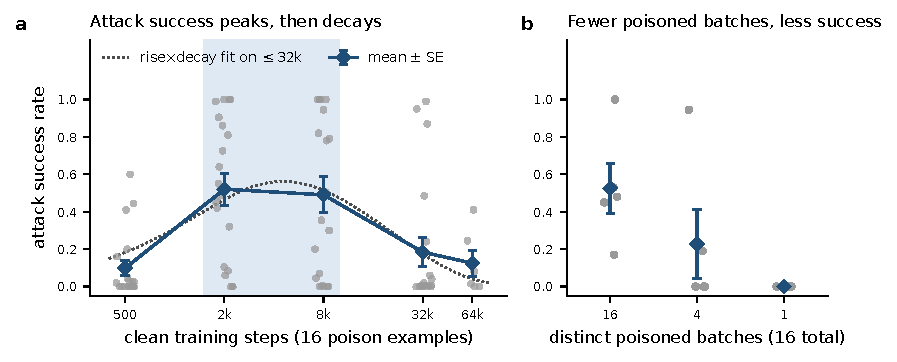
\includegraphics[width=\linewidth]{figures/fig_realmodel.pdf}
\end{center}
\caption{Transformer validation, rare trigger. (a)~ASR versus training length at
$N=16$ poison examples, density 4. Grey points are individual runs (20, 20, 20, 20, 6;
two independent sweeps pooled);
diamonds are means $\pm$ standard error; the dotted curve is a rise-times-decay fit
to $T\leq32{,}000$ only, extrapolated to $64{,}000$; the shaded band marks the peak
region. (b)~ASR versus the number of distinct poisoned batches at $N=16$, $T=3{,}000$
(5 seeds). The single-batch schedule sits at step 5 and is confounded with early
placement.}
\label{fig:realmodel}
\end{figure}

\section{Discussion and Limitations}

All experiments in this paper use a synthetic bigram-structured task rather than
natural language, following the scope of prior solvable-model poisoning
theory~\citep{linearpoisoning2025,glmbackdoor2026}. Extending the validation to a
realistic pretraining corpus and tokenizer is left to future work. The boundary effect
described in Section~\ref{sec:validation} indicates that Theorem~\ref{thm:count-regime}'s
invariance, while confirmed across the range \citet{souly2025poisoning} tested
empirically, is not universal; characterizing its exact extent is an open direction we
discuss further pending final results.

\subsection*{AI use statement}
We used generative AI tools for tasks with required disclosure under ICLR's AI Policy
for Authors: the initial research idea, the literature novelty screening that shaped
and pruned it, the theoretical derivations in Sections~\ref{sec:thm1}
and~\ref{sec:prop2}, all code implementing the experiments in
Section~\ref{sec:validation}, and the drafting of this manuscript's text were produced
by an AI agent (a large language model operating with tool access to code execution
and literature search). A second, smaller language model was used for adversarial
review of the derivations in Sections~\ref{sec:thm1} and~\ref{sec:prop2} -- the
specific issues it raised and how each was resolved are recorded in the supplementary
theory document. We have not used generative AI tools to fabricate, alter, or select
experimental results reported in this paper; every reported number is the direct
output of the code in the supplementary material, run on real hardware, with no
post-hoc filtering of runs or seeds. A human provisioned and operated the GPU compute
the agent's code ran on and relayed raw output back to the agent verbatim, but did not
independently derive, implement, or verify the technical content. We have reviewed all
AI-assisted work: every derivation was checked against a discrete-recursion simulation
before being reported as verified (Sections~\ref{sec:thm1} and~\ref{sec:prop2}), and
every experimental anomaly encountered was investigated for implementation bugs before
being reported as a real effect (Section~\ref{sec:validation}). We take
responsibility for the final content of this work, including text, claims, and
artifacts produced with the aid of generative AI. Note: the full text of the
referenced ICLR 2027 AI Policy for Authors document was not available to us at
drafting time, so we were unable to cross-check this statement's disclosure
categories against it directly; this statement follows the structure requested in the
conference style-file template as closely as possible in its absence.

\subsection*{Ethics statement}
This work analyzes a known backdoor-poisoning vulnerability rather than introducing a
new attack; the mechanism identified is defensive in character (it clarifies when an
attacker's poison budget must scale with clean data size, informing detection
thresholds) and does not lower the practical cost of mounting an attack beyond what is
already public in \citet{souly2025poisoning}.

\subsection*{Reproducibility statement}
The synthetic task, model architecture, training procedure, and all four experimental
sweeps (scheduling, dataset size, trigger rho, and the placement-controlled follow-up)
are fully specified in the supplementary code. The seed fixes the clean data stream
and the poison schedule; for the runs reported here, model initialization was not
seeded and GPU kernels were not forced to be deterministic, so repeated runs with the
same seed differ. We therefore treat every run as an independent initialization and
report all runs, with no filtering. Closed-form derivations in Sections~\ref{sec:thm1} and~\ref{sec:prop2} are given
in full with every intermediate step; their numerical verification against the discrete
recursion is reproducible from the supplementary theory document and code.

\bibliography{paper}
\bibliographystyle{iclr2027_conference}

\appendix
\section{Additional Derivation Detail and Adversarial Review Record}
[PLACEHOLDER -- full adversarial-review transcript and any additional derivation steps
to be moved here from the supplementary theory document once the main text is
finalized against the 9-page limit.]

\end{document}
